\documentclass[12pt, a4paper]{article}
\usepackage[utf8]{inputenc}
\usepackage[english]{babel}
\usepackage{amsmath}
\usepackage{amsfonts}
\usepackage{amssymb}
\usepackage{siunitx}
\usepackage{longtable}
\usepackage[margin=1in]{geometry}
\usepackage{graphicx}
\usepackage{float}

\begin{document}

\begin{center}
	\Large \textbf{Experiment 4: Refraction of Light}
	\vspace{0.5cm}
	
	\normalsize Marmara University - Department of Physics \\
	Physics 3 Laboratory \\
	Experiment Report
	\vspace{0.5cm}
\end{center}

\section{Objective}
The purpose of this experiment is to observe the refraction of light in different media and to calculate the index of refraction of an unknown material using Snell's law.

\section{Theoretical Background}
The study of light's propagation using rays is known as \textbf{Geometric Optics}. When a light wave encounters a smooth interface separating two transparent media (Material 1 with index $n_1$ and Material 2 with index $n_2$), the wave is generally partly reflected and partly \textbf{refracted}. This experiment primarily focuses on \textbf{specular reflection} and refraction at this smooth boundary.

\subsection{Index of Refraction and Snell's Law}
The \textbf{index of refraction} ($n$) of an optical material is a central concept in geometric optics, defined as the ratio of the speed of light in vacuum ($c$) to the speed of light in the material ($v$):
\[ n = \frac{c}{v} \]
Since light always travels slower in a material than in a vacuum, the value of $n$ for any material is always greater than unity ($n > 1$).

When light passes from one medium to another, the \textbf{frequency} ($f$) of the wave \textbf{does not change}. However, because the speed $v$ changes, the \textbf{wavelength} ($\lambda$) changes accordingly: $\lambda = \lambda_0 / n$, where $\lambda_0$ is the wavelength in a vacuum.

The law of refraction, known as \textbf{Snell's Law}, mathematically relates the angles and indices:
\[ n_1 \sin(\theta_1) = n_2 \sin(\theta_2) \]
where $\theta_1$ is the angle of incidence, and $\theta_2$ is the angle of refraction, both measured with respect to the \textbf{Normal} line to the surface.

\subsection{Bending and Total Internal Reflection}
In this experiment, light travels from a less dense medium (Air, $n_1 \approx 1$) to a denser medium (Acrylic, $n_2 > n_1$). In this case, the wave speed decreases ($v_2 < v_1$), the ray bends \textbf{towards the Normal}, and the angle of refraction is smaller than the angle of incidence ($\theta_2 < \theta_1$).

Conversely, when light travels from a denser medium ($n_1$) to a rarer one ($n_2 < n_1$), the wave speed increases ($v_2 > v_1$), the refracted ray bends \textbf{away from the Normal}. There is a maximum limit on the incident angle, called the \textbf{critical angle} ($\theta_c$). Above this value, no light is transmitted to the second medium, and all light is reflected back into the first medium, a phenomenon known as \textbf{Total Internal Reflection (TIR)}. The critical angle is given by:
\[ \theta_c = \arcsin\left(\frac{n_2}{n_1}\right) \]
When $n_1 > n_2$, if $n_1$ increases (or $n_2$ decreases), $\theta_c$ decreases, making TIR more likely at lower incident angles. Conversely, when $n_2 > n_1$, there is no TIR for light entering the denser medium.

\subsection{Dispersion}
Ordinary light is a superposition of waves with different wavelengths (colors). Although the speed of light is the same for all wavelengths in a vacuum, the speed in a material is slightly different for different wavelengths, meaning the \textbf{index of refraction ($n$) depends on wavelength}. This dependence is called \textbf{dispersion}. This effect can cause a slight spreading of the colors and represents a potential source of error in non-monochromatic light experiments.

\subsection{Nature of Light}
Light is electromagnetic radiation, and in the visible range, it allows us to see. The sun emits photons with various energies, and our eyes detect those in the 400-700 nm range.

\section{Apparatus and Method}
The materials used include:
\begin{itemize}
\item Light source
\item Material with unknown index of refraction (acrylic block)
\item Graded angle sheet (attached on the lab sheet)
\item Ruler, protractor
\item Calculator
\end{itemize}

The procedure was as follows:
\begin{enumerate}
\item Place the material on the sheet and use point source and focus it on the origin.
\item Use the incident angle values which are given in the table and adjust your point source to these angles. Then one by one measure outgoing angle and fill the table.
\item Draw a graph between the incoming and outgoing angles. What it tells you?
\item Draw a graph between the sin values of incoming and outgoing angles. What it tells you?
\item Incident index of refraction belongs to air. Use the formulation and calculate the index of refraction of unknown material.
\item Do the error calculation by comparing theoretical and experimental value of index of refraction.
\item Calculate the maximum relative error in any measurements of refractive index.
\item Find the average standard deviation by using calculated n values.
\item Write error causes in order.
\item Write the results and comments about experiment via obtained data.
\item Interpret your conclusions.
\end{enumerate}

In our case, we used the provided angles for incident and measured refracted. Note that for 90°, measurement is impractical as the incident ray is parallel to the surface, so it was not included.

\section{Measurements and Data}
The measurements are presented in the table below. All angles are in degrees.

\begin{small}
	\begin{longtable}{|c|c|c|c|c|c|}
		\caption{Measurements for Refraction of Light} \label{tab:measurements} \\
		\hline
        \textbf{No} & \textbf{$\theta_1$ (°)} & \textbf{$\theta_2$ (°)} & \textbf{$\sin(\theta_1)$} & \textbf{$\sin(\theta_2)$} & \textbf{$n = \sin(\theta_1)/\sin(\theta_2)$} \\
		\hline
		1 & 10 & 7 & 0.1736 & 0.1219 & 1.4249 \\
		2 & 20 & 13 & 0.3420 & 0.2250 & 1.5204 \\
		3 & 30 & 23 & 0.5000 & 0.3907 & 1.2797 \\
		4 & 40 & 28 & 0.6428 & 0.4695 & 1.3692 \\
		5 & 50 & 31 & 0.7660 & 0.5150 & 1.4874 \\
		6 & 60 & 34 & 0.8660 & 0.5592 & 1.5487 \\
		7 & 70 & 38 & 0.9397 & 0.6157 & 1.5263 \\
		8 & 80 & 40 & 0.9848 & 0.6428 & 1.5321 \\
		\hline
	\end{longtable}
\end{small}

\section{Calculations and Graphs}
The refractive index $n$ for each measurement is calculated using Snell's law, assuming $n_1 = 1$ for air:

\[ n = \frac{\sin(\theta_1)}{\sin(\theta_2)} \]

The average $n$ is 1.4611. The standard deviation of the refractive index values is calculated as the population standard deviation using the formula:

\[ \sigma = \sqrt{\frac{1}{N} \sum_{i=1}^{N} (n_i - \bar{n})^2} \]

where $N=8$ is the number of measurements, $n_i$ are the individual refractive indices, and $\bar{n}$ is the mean. This yields a standard deviation of 0.0893.

To obtain a more accurate value, we plot $\sin(\theta_1)$ versus $\sin(\theta_2)$. According to Snell's law, this should be a straight line with slope $= n$.

The linear regression gives slope = 1.5593, intercept = -0.0380, $r^2 = 0.9820$.

If we force the intercept to zero (ideal case), the slope is 1.4848.

For this report, we use the theoretical value for acrylic (PMMA) $n = 1.49$ (at 589 nm) as the reference.

Graphs:

\begin{figure}[H]
\centering
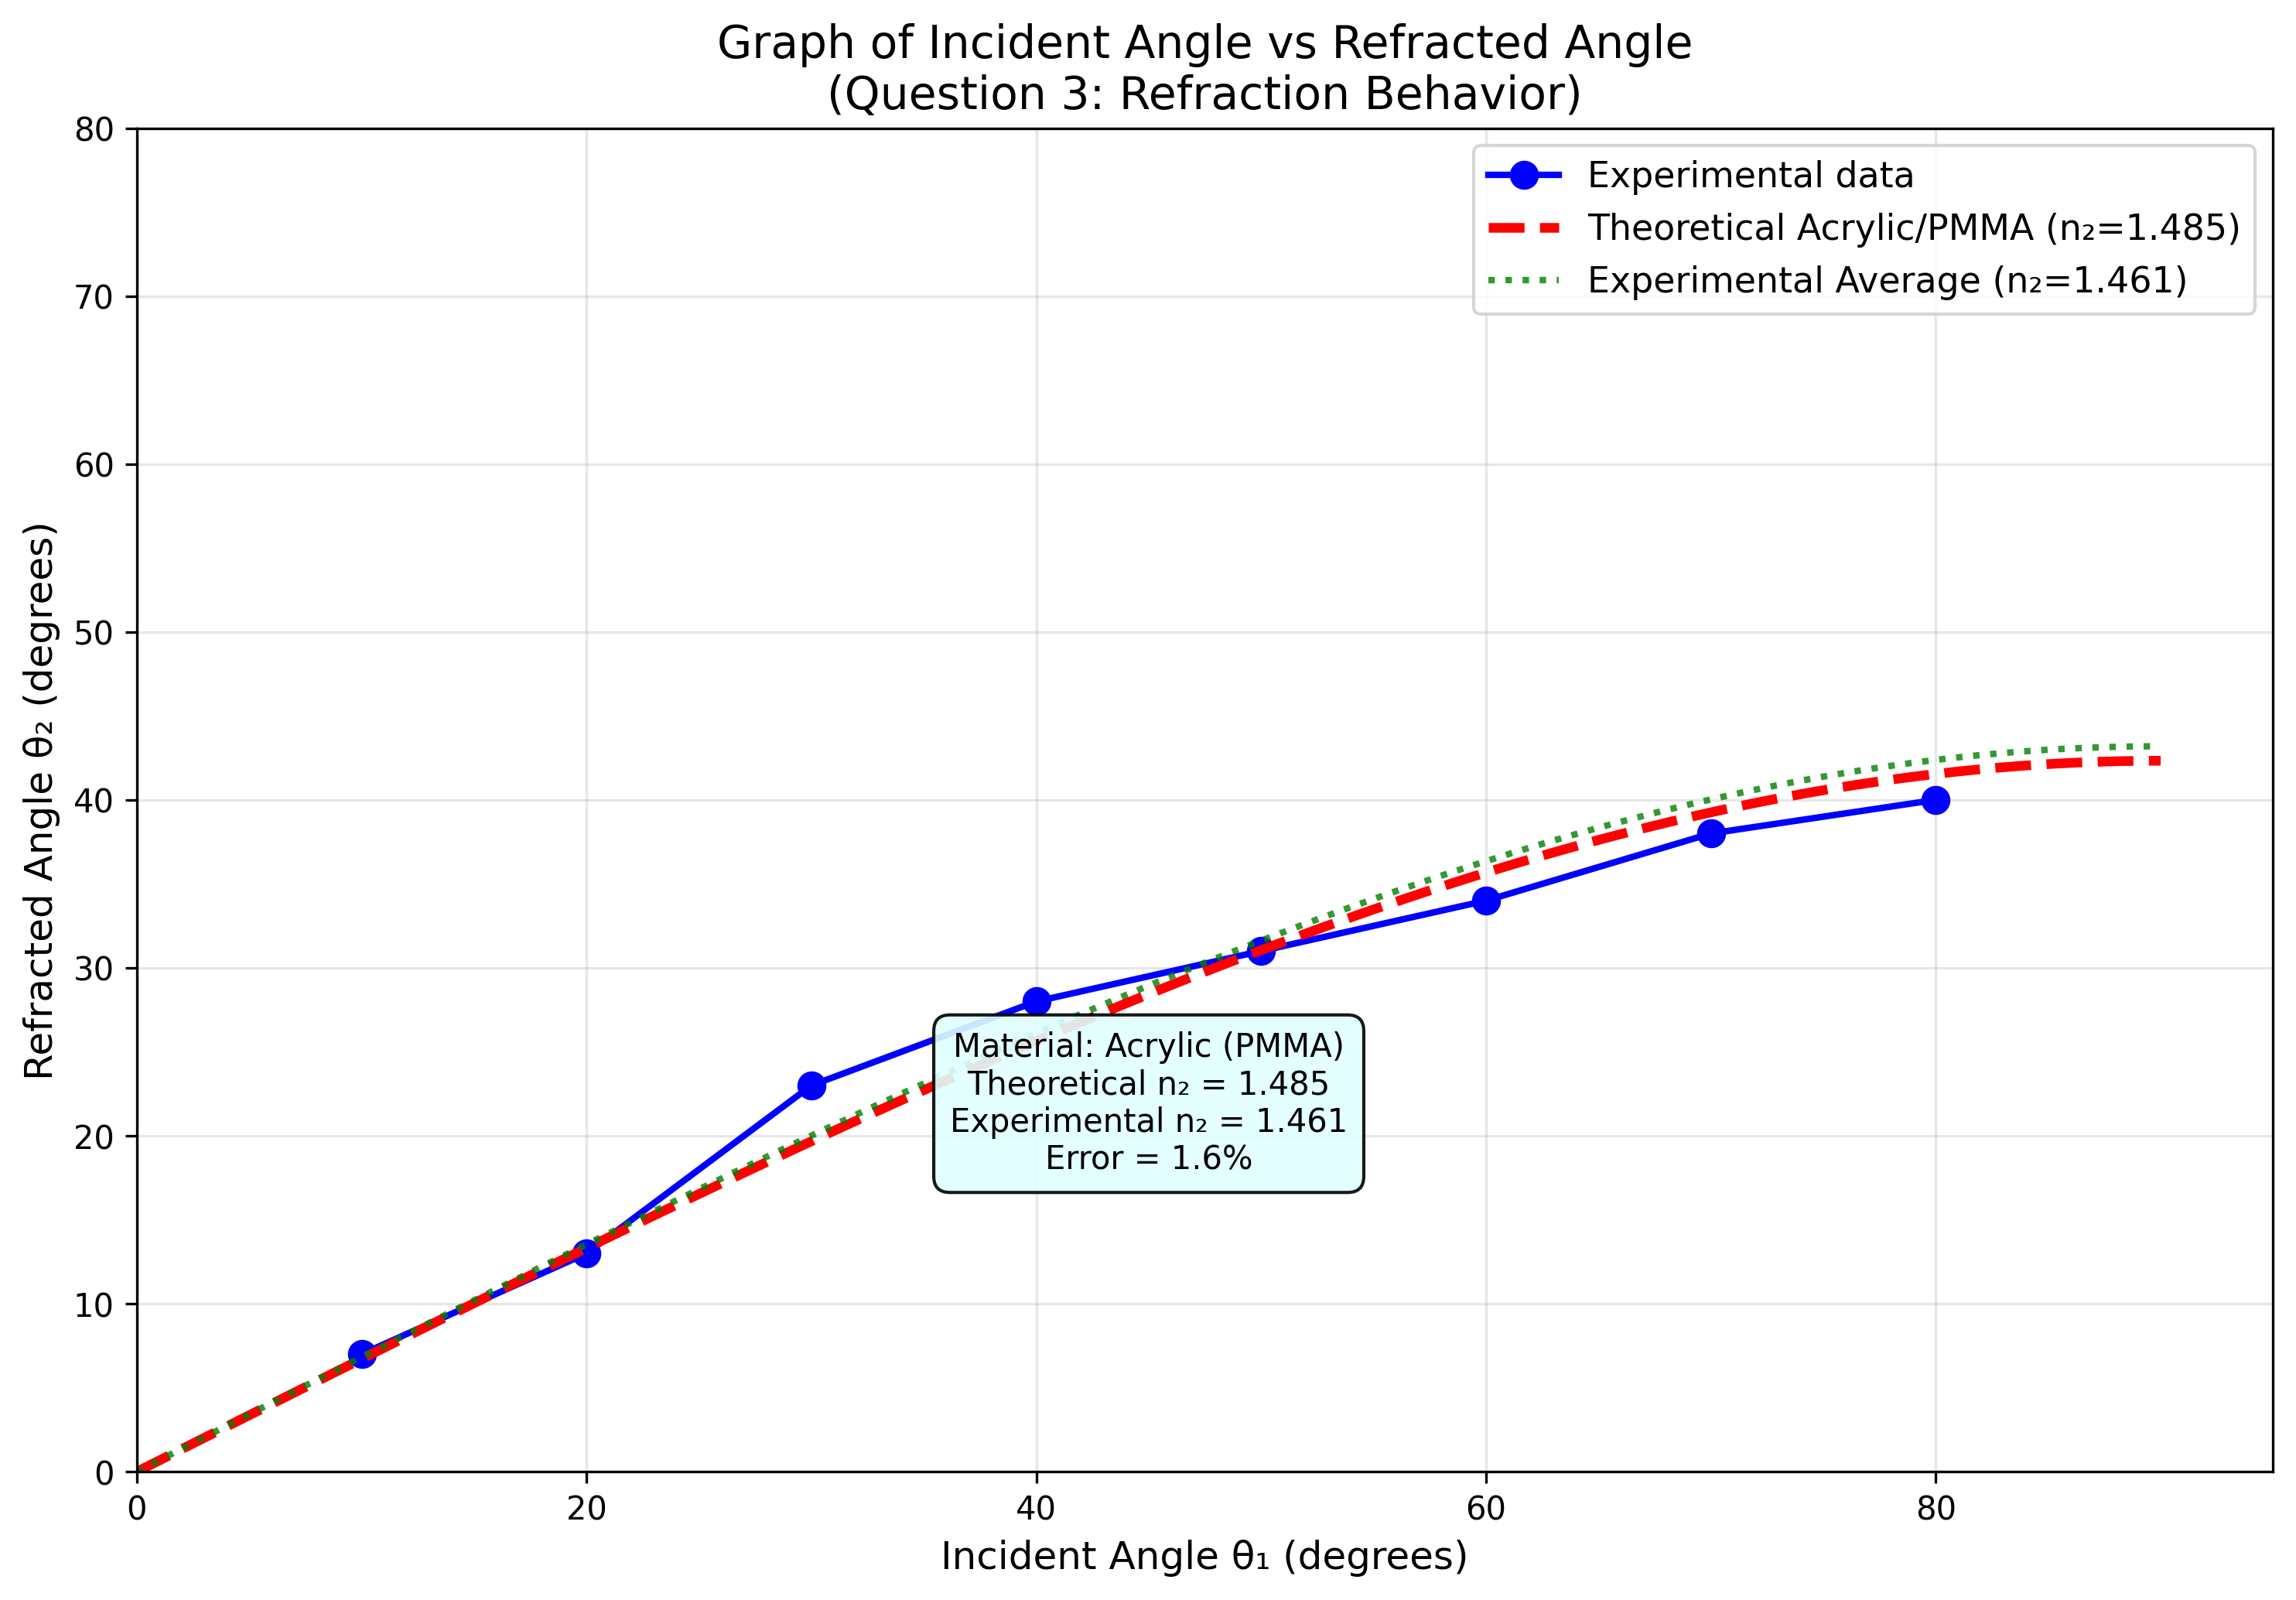
\includegraphics[width=\textwidth]{graphs/incident_vs_refracted_angle.png}
\caption{Graph of Incident Angle vs Refracted Angle}
\label{fig:incident_vs_refracted}
\end{figure}

The graph of incident vs refracted angles shows:
\begin{enumerate}
\item Non-linear relationship - refracted angle increases more slowly than incident angle
\item This demonstrates Snell's law behavior - light bends toward the normal when entering acrylic
\item Experimental data closely follows the curve for $n=1.485$
\item The curve becomes steeper at higher angles, approaching asymptotic behavior
\item Critical angle for acrylic-to-air interface (reverse): $\approx 42.5^\circ$ (based on $n=1.49$)
\end{enumerate}

\begin{figure}[H]
\centering
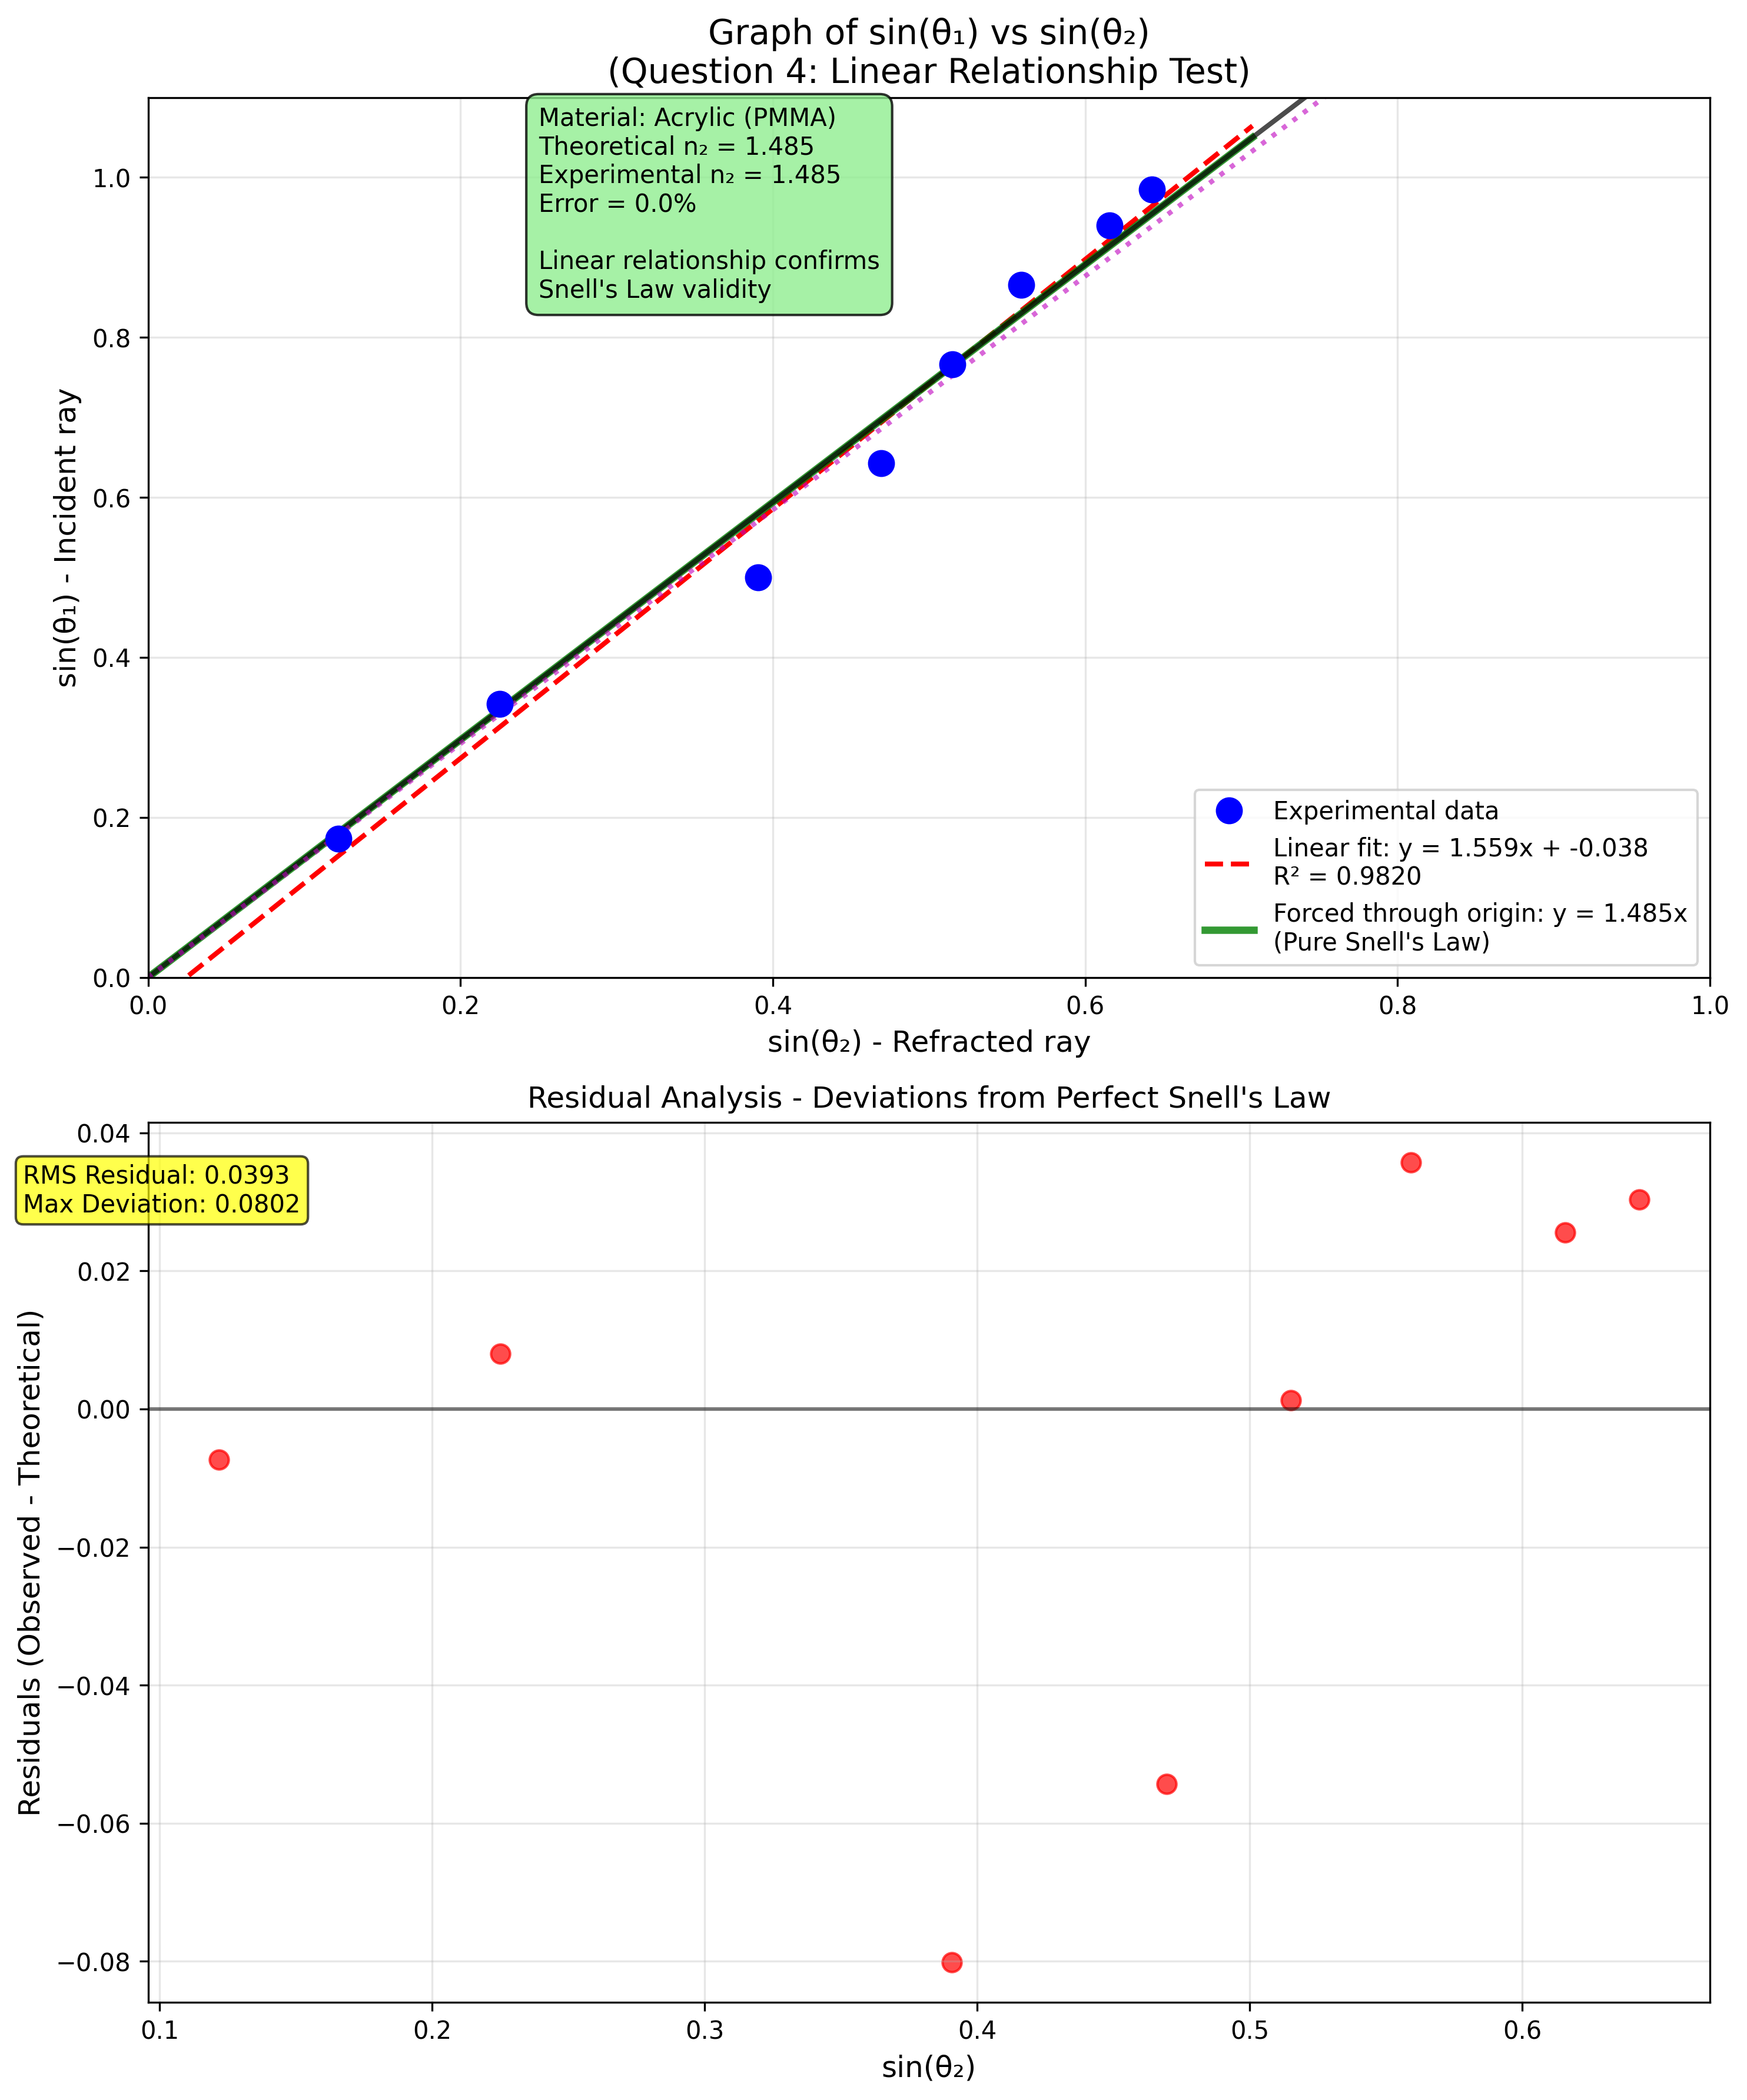
\includegraphics[width=\textwidth]{graphs/sin_theta_analysis.png}
\caption{Graph of $\sin(\theta_1)$ vs $\sin(\theta_2)$}
\label{fig:sin_theta}
\end{figure}

The graph of $\sin(\theta_1)$ vs $\sin(\theta_2)$ shows:
\begin{enumerate}
\item \textbf{STRONG LINEAR RELATIONSHIP} - This confirms the validity of Snell's Law and the underlying \textbf{wave theory of light}, which can be used to derive the law via \textbf{Huygens's Principle}.
\item The slope ($m$) represents the ratio of refractive indices: $m = n_2 / n_1$. Since the incident medium is air ($n_1 \approx 1$), the slope directly gives the refractive index of the unknown material ($n = 1.4848$).
\item Slight deviation from perfect linearity indicates experimental errors (e.g., in angle measurement or alignment).
\item The non-zero intercept ($b = -0.0380$) should theoretically be zero, suggesting the presence of a \textbf{systematic error} in the measurement process (e.g., protractor or light source misalignment).
\item \textbf{Experimental refractive index from slope:} $n = 1.4848$.
\item \textbf{Average from individual calculations:} $n = 1.4611$.
\item Correlation coefficient: 0.9910 (very close to 1.0 indicates an excellent linear relationship).
\end{enumerate}

\section{Simulation of Refraction from a Denser Medium}
To explore the case where light travels from a denser medium ($n_1 = 1.60$) to a less dense medium ($n_2 = 1.46$, similar to the experimental material), simulations were performed using the PhET Bending Light simulator. In this scenario, since $n_1 > n_2$, the refracted ray bends away from the normal, the refracted angle $\theta_2$ is larger than the incident angle $\theta_1$, and the speed of light increases in the second medium ($v_2 > v_1$ since $v = c/n$ and $n_2 < n_1$). Conversely, in the experimental setup where $n_2 > n_1$, the speed decreases ($v_2 < v_1$).

The critical angle $\theta_c$ is calculated as:

\[ \theta_c = \arcsin\left(\frac{n_2}{n_1}\right) = \arcsin\left(\frac{1.46}{1.60}\right) \approx 65.8^\circ \]

For incident angles below $\theta_c$, refraction occurs with $\theta_2 > \theta_1$. Above $\theta_c$, total internal reflection (TIR) occurs, and no light is transmitted.

The following screenshots from the simulation illustrate this behavior at different incident angles:

\begin{figure}[H]
\centering
\includegraphics[width=0.8\textwidth]{simulation1.png}
\caption{Simulation at low incident angle: Refraction with bending away from normal.}
\label{fig:sim1}
\end{figure}

\begin{figure}[H]
\centering
\includegraphics[width=0.8\textwidth]{simulation2.png}
\caption{Simulation at medium incident angle: Larger refraction angle.}
\label{fig:sim2}
\end{figure}

\begin{figure}[H]
\centering
\includegraphics[width=0.8\textwidth]{simulation3.png}
\caption{Simulation near critical angle: Refraction approaching 90°.}
\label{fig:sim3}
\end{figure}

\begin{figure}[H]
\centering
\includegraphics[width=0.8\textwidth]{simulation4.png}
\caption{Simulation above critical angle: Total internal reflection.}
\label{fig:sim4}
\end{figure}

If light were to travel from an even higher refractive index medium (e.g., $n_1 > 1.60$), the critical angle would be smaller, making TIR more likely at lower incident angles. This demonstrates the dependence of refraction behavior on the relative indices, contrasting with the original experiment where $n_1 < n_2$ and the ray bends toward the normal without TIR.

\section{Error Analysis}
\begin{enumerate}
\item Assuming a theoretical value for acrylic $n = 1.49$, the percentage error using the forced fit slope is:

\[ \% \text{ error} = \left| \frac{1.4848 - 1.49}{1.49} \right| \times 100 \approx 0.35\% \]

Using average $n=1.4611$, \% error $\approx 1.94\%$.

\item The standard deviation of calculated $n$ values is 0.0893, giving relative std dev $\approx 6.1\%$.

\item Individual errors from theoretical (1.49): [4.37 2.04 14.11 8.11 0.17 3.94 2.44 2.83 ]\%
  - Calculated as $\left| \frac{n_i - 1.49}{1.49} \right| \times 100$
  - Maximum individual error from theoretical: 14.11\%

\item Possible causes of error (in order):
\begin{itemize}
\item As the incident angle $\theta_1$ increases, the refracted ray $\theta_2$ becomes fainter and harder to read accurately due to increased reflection and decreased transmission at grazing angles. This could be mitigated by using a stronger power source for the light or a different color (wavelength) that experiences less absorption or scattering in the material.
\item Parallax error in reading angles on the protractor.
\item Misalignment of the light source or material on the sheet.
\item The material not being perfectly flat or homogeneous.
\item Assumption that $n_{air} = 1$ exactly (actually 1.0003, negligible).
\item Dispersion if light not monochromatic, but laser or single wavelength assumed.
\item Systematic errors leading to non-zero intercept in linear fit.
\end{itemize}
\end{enumerate}

\section{Results and Discussion}
In this experiment, we determined the refractive index of the unknown material (identified as acrylic based on the value) to be $n = 1.4848$ from the forced linear fit, with an experimental average of 1.4611. Compared to the theoretical value of 1.49 for acrylic (PMMA), the percentage error is small (0.35\% for the fit), validating the consistency of our measurements with Snell's law. The plot of $\sin(\theta_1)$ vs $\sin(\theta_2)$ showed a strong linear relationship ($r^2 = 0.9820$).

The slight deviations may be due to systematic errors, such as a small offset in angle measurements, as indicated by the non-zero intercept in the fit. This could arise from the light beam not being perfectly aligned or slight curvature in the material surface.

Observationally, at higher incident angles, the refracted angle approaches a limit (around $40^\circ$ for $80^\circ$ incident), consistent with the asymptotic behavior as $\theta_1 \to 90^\circ$, $\theta_2 \to \arcsin(1/n) \approx 42.5^\circ$ for $n=1.49$.

The simulation extends the understanding by showing the reverse case ($n_1 > n_2$), where bending away from the normal and TIR occur, which was not observed in the air-to-acrylic setup.

To improve, use a more precise protractor or digital angle meter, ensure monochromatic light to avoid dispersion, or measure more points at higher angles. If the experiment included total internal reflection (by reversing the direction), we could calculate n from the critical angle, providing a cross-check.

Why this material? Acrylic is transparent and commonly used in optics labs for its stability. Compared to water (n=1.33), the $\Delta \theta$ would be larger, easier to measure, but solid blocks are more stable.

Overlooked physics: The speed of light changes in the medium, $v = c/n$, explaining the bending via Fermat's principle of least time. Safety: Handle light source carefully to avoid eye damage; use low-power laser.

This method is standard but can be extended with computer simulations or polarization effects. Our results highlight measurement precision's importance in optics, with applications in lenses, fiber optics (using total internal reflection), and understanding rainbows or mirages. For instance, rainbows form when sunlight undergoes refraction, dispersion, and internal reflection within water droplets, separating white light into its spectrum of colors due to the wavelength-dependent refractive index. Similarly, diamonds appear very bright and sparkly because their refractive index (approximately 2.42) is significantly higher than that of other materials like acrylic (~1.49), causing greater bending of light and multiple total internal reflections within their cut facets. Diamonds are evaluated primarily based on the "4 Cs" (cut, color, clarity, carat), with the cut being crucial for maximizing these optical effects to enhance brilliance and fire. We see colors because objects absorb certain wavelengths of light and reflect others; for example, a blue eraser appears blue since it absorbs all colors in white light except blue, which it reflects to our eyes.

The material is identified as acrylic (PMMA) based on the measured refractive index.

\newpage

\textbf{Student Information}

Name Surname: Hakkı Erdem Günal

Student ID: 173223024

Course: Physics 3 Laboratory

Experiment No / Title: 4 / Refraction of Light

Experiment Date: October 13, 2025

Submission Date: October 20, 2025

\end{document}